%!TEX root = main.tex
\chapter{Contributions}
\chaptertable
\section{Introduction}
Les \gls{EVC3D} doivent considérer beaucoup de critères pour proposer un 
système réactif, robuste et permettant le passage à l'échelle en intégrant les 
contraintes liées à la gestion de données \gls{3D}. La dimension collaborative 
ajoute les problématiques de gestion de données concurrentes.
S'intéresser d'abord aux spécificités liées à l'assemblage d'objets \gls{3D} dans 
une scène partagée permet de mieux comprendre les fonctionnalités spécifiques à 
la \gls{3D} (transformations), à l'historique et à la visualisation des données. 
De plus, les données générées doivent suivre un flux de validation avant d'être 
intégrées totalement au système.
Les ressources nécessaires à la collaboration demandent une haute disponibilité 
et une forte réactivité qui implique la modélisation d'une architecture 
de communication répondant aux contraintes fonctionnelles (détection de conflit) 
et technologiques (web).

Ce chapitre détaille les contributions scientifiques de cette thèse.
Tout d'abord, il présente le modèle orienté événements pour la visualisation et la 
manipulation d'objets \gls{3D} dans un environnement web. 
Cette première contribution insiste sur l'intégration de la partie métier de la 
\gls{3D} par l'utilisation des patrons de conception \gls{DDD}, \gls{CQRS} et 
\gls{ES}. 
La réflexion concernant le découpage des opérations \gls{3D} liées à la 
manipulation d'objets \gls{3D} est d'abord expliquée ; puis, pour procurer plus 
d'autonomie aux utilisateurs, la contribution intègre le fait de déporter le patron 
\gls{CQRS} uniquement sur le client afin qu'il soit capable de gérer la partie métier 
seul. La valeur ajoutée par le modèle orienté événements est l'intégration des 
aspects métiers de la modélisation 3D des actions des utilisateurs à la 
visualisation. 

La seconde contribution de cette thèse concerne l'architecture de 
communication dans un environnement web. Celle-ci doit permettre au système 
d'être résilient, léger et transparent. 
L'architecture hybride proposée repose sur une combinaison de l'architecture 
client-serveur et l'architecture \gls{P2P}. 
Cela tient à la nécessaire centralisation de l'information dans un contexte industriel 
et à la haute disponibilité des ressources que permettent les propriétés du 
\gls{P2P}. Cette contribution est découpée en deux parties. 

La première expose une preuve de concept, sur la base du modèle présenté dans 
\cite{Desprat2015a}, avec une architecture de communication simple proposant 
une diffusion des mises à jour par différentiel d'état. La seconde partie 
tire avantage de la mise en place du \gls{framework} orienté événements présenté 
dans \cite{Desprat2016} et utilise la méthode de distribution des informations 
présenté dans \cite{Desprat2017} pour améliorer la résilience du système. 

%%%%%%% SECTION %%%%%%%
%\section{Modèle événementiel pour l'intégration du domaine 3D lors de la 
%manipulation d'objets 3D}
%!TEX root = main.tex

%%%%%%% SECTION %%%%%%%
\section{Modèle évènementiel pour l'intégration du domaine 3D lors de la 
manipulation d'objets 3D}

%\subsection{Introduction}

L'\gls{EP} occupe, dans le champ de l'informatique, une place centrale dans 
beaucoup de systèmes comme l'énergie, la santé, l'environnement, les transports, 
la finance, les services et l'industrie. L'\gls{EP} réunit des méthodes et des outils 
pour filtrer, transformer, et détecter des motifs dans des évènements, dans le but 
de réagir à des conditions qui changent, généralement liées à des contraintes de 
temps \cite{Chandy2011}. L'\gls{EP} intègre plusieurs fonctionnalités:
\begin{itemize}
	\item Obtenir des données à partir de plusieurs sources en temps (quasi) réel
	\item Agréger et analyser ces données pour détecter des motifs qui indiquent la 
	présence de situation critiques qui nécessitent une réponse
	\item Déterminer la réponse la plus adaptée à ces situations
	\item Surveiller (\textit{monitor}) l'exécution de cette réponse
\end{itemize}

Le panorama d'applications et de technologies proposé par \cite{Hinze2009} 
permet de définir les termes et les interprétations communes à différents 
domaines se basant sur le paradigme de l'\gls{EP}. 


La méthodologie orientée évènements intègre plusieurs aspects souvent laissés 
de côté dans la littérature concernant le développement les environnements 
virtuels collaboratifs pour la visualisation et la manipulation d'objets 3D. Par 
exemple, elle a l'avantage de proposer un couplage lâche. Dès lors, la réutilisation 
des données produite lors de la collaboration peut facilement être réutiliser pour un 
traitement secondaire comme la sensibilisation aux éléments de l'environnement. 

%L'intégration de la partie métier L'un des aspects principaux a été de 
%combiner tous les aspects reliés aux évènements dans le \textit{pipeline} de 
%visualisation et de manipulation d'objets 3D. 
Le découpage de la modélisation logicielle et l'abstraction qu'elle apporte est aussi 
l'occasion de s'intéresser à la façon dont sont générées les données produites par 
les utilisateurs et la façon dont elles sont affichées. 

\subsubsection{Constat}

Par nature, une architecture orientée évènements est extrêmement peu couplée et 
hautement distribuée. Le créateur de l'évènement sait seulement que l'évènement 
se produit. 
Le créateur de l'évènement n'a aucune idée du traitement l'évènement va subir par 
la suite ou qui cela va concerner. La traçabilité peut donc devenir difficile lorsqu'un 
évènement empreinte de multiples chemin. C'est pourquoi les architectures 
orientée évènements sont plus utilisées dans un contexte de flux d'information 
asynchrone. 

Il existe différent types de traitement d'évènement : simple, en continu, complexe. 
Ils peuvent être utilisés ensemble dans le cadre.
\begin{itemize}
\item Traitement d'évènement simple. (\textit{simple event processing}). 
Dans le traitement simple d'évènement, un évènement notable arrive, initiant une 
cascade d'actions. Le traitement simple d'évènement est généralement utilisé pour 
orienter un flux temps-réel qui peut prendre un peu de temps, n'entraînant pas de 
coût sur la partie métier.
\item Traitement de flux continu d'évènement. (\textit{stream event 
processing}). 
\item Traitement d'évènement complexe. (\textit{complex event 
processing}). 

\end{itemize}

Le choix de baser la gestion des données sur le patron de conception \gls{CQRS} 
combiné à de l'\gls{ES} repose sur le constat suivant: dans un cadre industriel, le 
besoin de traçabilité de l'information est très important. 

\gls{CQRS} est principalement utilisé sur des applications \gls{CS} qui sont 
toujours connectées (pour récupérer les mises à jour). Ce fonctionnement ne 
permet pas le travail hors ligne.

Côté serveur, le stockage des données est de moins en moins cher, on peut donc 
se permettre de stocker beaucoup de données de manière distante notamment 
grâce au \gls{cloud}\info{definir le cloud}. Le serveur a une puissance de calcul 
plus importante (et surtout ajustable).

Côté client, la puissance de calcul des machines sur lesquelles sont installés les 
navigateurs web évolue rapidement (notamment les appareils mobiles comme les 
\textit{smartphones} et les tablettes). Les navigateurs suivent cette tendance en 
puisant dans ces ressources pour effectuer des traitements similaires à ceux que 
l'on trouve côté serveur traditionnellement et pour proposer des fonctionnalités 
avancées telles que le stockage important de données sur le client (IndexedDB, 
storageAPI), pour l'affichage 3D (WebGL) et pour la communication en \gls{P2P} 
(\gls{WebRTC}). En déportant ainsi la charge que pourrait subir une architecture 
traditionnelle client-serveur côté client, les échangent réseaux sont limités car qui 
sont très coûteux d'un point de vue énergétique pour les appareils mobiles 
\cite{Koskela2015}. De plus, l'utilisation de la bande passante est onéreuse et 
parfois limitée voire inexistante, il est donc nécessaire de tirer parti de tous les 
appareils participants à la collaboration au lieu de tout faire reposer sur le serveur. 
Chaque appareil participant à la collaboration doit être autonome et le plus 
indépendant possible en termes de ressources (données, réseaux, validation 
experte). 


\subsubsection{Contribution}
Pour répondre à cette problématique, nous proposons une solution pour la 
transmission des données 3D et collaboratives qui permet de  limiter  le nombre 
de requêtes et la taille des données transmises sans perdre la traçabilité de 
celles-ci. L'idée est de profiter de la puissance du client pour créer une 
architecture assurant l'autonomie de l'utilisateur en cas de déconnexion volontaire 
(travaille hors ligne) ou involontaire (coupure). On garantit ainsi à l'utilisateur 
l'utilisation du système avec un historique performant où chaque connexion est 
l'occasion de mettre le système à jour.


\subsection{Modèle général}
La composition de l'architecture s'est effectuée avec en arrière pensée les lignes 
directrices données par  énoncées plus haut\info{ref section} \cite{Xhafa2010}. 
Utiliser une architecture orientée évènements pour faire de la modélisation 3D peut 
sembler non nécessaire. Cependant lorsqu'on s'intéresse aux apports que cela 
peut générer pour tous les métiers engagés (utilisateurs, développeurs, analystes 
métier) on peut se demander pourquoi cela n'a pas été plus mis en avant 
auparavant. La sensibilisation à l'historique des données et aux interactions 
inter-utilisateurs est partagée  par les utilisateurs et les analystes métier. Quand à 
la sensibilisation à la distribution des données elles est une composante 
importante pour les utilisateurs et les développeurs. Concernant les premiers, cela 
garantie une certaine autonomie dans la création. Pour les seconds, la répartition 
de la charge permet de profiter du potentiel computationnel de toutes les parties 
prenantes du réseau. 

Dans 3DEvent, le langage partagé se réfère au domaine de la manipulation 
d'objets 3D mais aussi au domaine de la collaboration. Par exemple le terme de 
maillage peut se référer à la fois au maillage géométrique ou bien au maillage de 
l'architecture réseau, d'où l'importance de définir les différents contextes en amont. 
Notons que le contexte de l'application peut faire varier les frontières d'un 
domaine. Le modèle issu du domaine défini permet de mettre en valeur les 
aspects métiers liés à l'application.



Le patron \glsreset{ES}\gls{ES} permet de capturer tous les changements d'état 
d'une application sous la forme d'une séquence d'évènements. 
Ces évènements sont conservés dans un journal d'évènements et peuvent être 
rejoués pour retrouver l'état de l'application. 
Les évènements représentent des faits immuables qui sont 
seulement ajoutés au journal les un après les autres, ce qui permet des taux de 
transaction élevés et une réplication efficace (cf Section 
\ref{sec:es}). Dans 3DEvent, plusieurs composants d'\gls{ES} sont étendues selon 
les applications :

\begin{description}
	\item[Acteur] Un acteur consomme des évènements à partir d'un journal 
	d'évènements et produit des évènements pour le même journal d'évènements. 
	L'état interne dérivé à partir des évènements consommés est un modèle 
	d'écriture 
	en mémoire (\textit{in-memory}) et contribue à la partie commande (C) du 
	CQRS\info{reference à la section}.
	\item[Vue] Une vue est un acteur qui ne fait que consommer des évènements à 
	partir du journal d'évènement. L'état interne dérivé à partir des évènements 
	consommés est un modèle de lecture en mémoire et contribue à la partie 
	requête (Q) du CQRS\info{reference à la section}.
	\item[Producteur] Un producteur est un acteur qui produit des évènements à 
	partir 
	du journal d'évènements pour mettre à jour la base de données. L'état interne 
	dérivé 
	à partir des évènements consommés est un modèle de lecture en mémoire et 
	contribue à la partie requête (Q) du CQRS\info{reference à la section}.
	\item[Processeur] Un processeur est un acteur qui consomme des évènements 
	à 
	partir d'un journal d'évènements et produit les évènements traités pour un autre 
	journal d'évènements. Les processeurs peuvent être utilisés pour connecter les 
	journaux d'évènement au traitement des évènements.\info{reference à la 
	section}.
	
\end{description}

%\subsubsection{Collaboration évènementielle}

Les évènements produits par un des composants présentée ci-dessus
peuvent être consommés par d'autres de ces abstractions s'ils partagent un 
journal d'évènements local ou distribué. 

Un journal d'évènements peut fonctionner sur un seul site ou alors être répliqué sur 
plusieurs sites. Le site est considéré comme une zone disponible qui accepte 
l'écriture d'un journal d'évènements local même s'il est partitionné sur plusieurs 
sites. Les journaux d'évènements locaux situés sur plusieurs sites peut être 
connectés par le biais d'un journal d'évènements dit \og repliqué\fg{} qui a pour 
responsabilité de préserver l'ordre causal des évènements.

Les sites peuvent être situés à des endroits géographiquement distincts ou sur 
des nœuds à l'intérieur d'une même grappe (\textit{cluster}) ou encore être sur le 
même nœud mais traités séparément selon les zones disponibles nécessaires au 
fonctionnement de l'application. Les Acteurs et les Processeurs écrivent 
cependant toujours sur leur journal d'évènements local. Les composants peuvent 
soit collaborer sur un journal d'évènements local sur le même site, ou bien au 
travers d'un journal répliqué sur différents sites.

Il est important de différencier le journal d'évènements de la base de données 
(côté serveur). 
La base de données peut ne contenir qu'une partie du journal. Une base de 
données peut également être considérée comme un élément complémentaire au 
journal d'évènements, cependant et bien que parfois confondus, ils restent bien 
distincts conceptuellement.

Le journal d'évènements commun est la base des échanges pour communiquer 
par le biais d'évènements de collaboration. Ce type d'architecture se retrouve dans 
différents cas d'utilisation :
\improve{est ce que cette section est nécessaire?}
\begin{itemize}
	\item \textit{Processus métier distribués.} Les acteurs de différents types 
	utilisent des évènements pour communiquer et parvenir à résoudre un problème 
	commun. Bien qu'ils jouent des rôles différent dans le processus métier, ils 
	réagissent à la réception d'évènements (\textit{reactive programming}) en 
	mettant à jour l'état de l'application et en produisant de nouveaux évènements. 
	Cette forme de collaboration est appelée collaboration dirigée par les 
	évènements.\improve{ref}
	\item\textit{Réplication d'état d'Acteur.} Les acteurs de même type consomme 
	les évènements de chacun pour répliquer l'état interne avec une cohérence 
	causale. Dans 3DEvent, les opérations concurrentes sont autorisées dans pour 
	mettre à jour l'état des acteurs répliqués et permettre la résolution interactive de 
	conflit en cas de mises à jour concurrentes et conflictuelles. \improve{miuex 
	expliquer}
	\item \textit{Agrégation d'évènement.} Les vues et les producteurs agrègent des 
	évènements a partir d'autres composants pour générer des vues spécifiques à 
	l'application.
	La collaboration évènementielle apporte de la fiabilité dans la gestion des 
	données dans un système distribué. Par exemple, si un processus distribué 
	échoue à cause d'un problème sur une partie du réseau, le système reprend 
	automatiquement dès les répliques sont à jour.
\end{itemize}

%\paragraph{Bus d'évènement}
Les composants souscrivent à leur journal d'évènements en s'accrochant au bus 
d'évènements. 
Les évènements nouveaux sont poussés vers les souscripteurs, 
ce qui leur permet de mettre à jour l'état de l'application avec une latence 
minimale. 
Un évènement écrit à un endroit est publié de manière fiable aux souscripteurs sur 
ce site et aux souscripteurs des sites distants. 
Par conséquent, les composants qui échanges par le biais d'un 
journal d'évènements répliqué communiquent via un bus qui préserve l'ordre causal 
des évènements de manière durable et tolérant au partitionnement. De ce fait, les 
services sur les partitions du réseau inter-sites (lien entre les sites) peuvent 
continuer d'écrire des évènements localement. La livraison des évènements sur 
les sites distants reprend automatique lorsque les partitions sont à jour.


Le journal d'évènements répliqué localement et fournit un ordre total des 
évènements stockés et appartient à un site. 
Le site est une zone de disponibilité qui héberge un ou plusieurs 
journal d'évènements. Les évènements d'un journal d'évènements sont 
répliqués de manière asynchrone sur les autres des journaux d'évènements 
des sites distants. 
Afin de lier des journaux d'évènements (localisés sur différents sites) à un journal 
d'évènements répliqué, les 
journaux d'évènements locaux doivent être accessibles à partir des points 
d'entrées de réplication. De plus, ces points d'entrée doivent être 
connectés entre eux afin de créer un réseau de réplications. 
Un journal d'évènements répliqué est représenté par un journal d'évènements local 
sur chacun des sites participants.

\info{point d'entrée = network bridge}

Les points d'entrée permettent de gérer un ou plusieurs journaux d'évènements. 
Ces journaux sont identifiés pour permettre à la réplication de ne s'intéresser 
qu'aux journaux de même identifiant. 
Les journaux avec différents identifiants sont ainsi isolés les uns des autres et 
leur distribution peut donc varier selon les sites.

Les journaux répliqués fournissent l'ordre causal des évènements stockés : l'ordre 
de stockage est le même sur tous les sites, ce qui veut dire que les 
consommateurs qui lisent les évènements du journal local vont toujours voir les 
effets avant leurs causes.




\subsection{Mécanisme de gestion de version}
3DEvent intègre une procédure de gestion de version dans l'\gls{EventStore} afin 
de gérer au mieux la cohérence des données. 
Chaque gestion de commande (Figure \ref{fig:gestionCommande}) entraîne la 
génération d'un ou plusieurs évènements. Ces évènements sont considérés 
comme \og soumis\fg{} (\textit{uncomitted}) mais pas encore <<~publiés~>> 
(\textit{comitted}).  Pour qu'ils le deviennent, l'agrégat concerné par ces 
évènements doit produire une nouvelle version sans être en conflit avec la 
précédente. En passant la version attendue $v_a$ au gestionnaire de conflit, on 
est à même de la comparer avec la version courante $v_c$. Il existe deux cas où 
un conflit est levé~: 
\begin{enumerate}[label=\alph*)]
	\item \label{i:vi} La version $v_a$ correspond à la valeur d'initialisation
	\item \label{i:vdiff} La version $v_a$ est différente de la version $v_c$
\end{enumerate}
Dans \ref{i:vi}, on s'assure qu'après une action la version initiale de l'agrégat ne 
peut être la même. Cet item peut sembler évident mais il est important de le noter 
car il dépend entièrement la valeur initiale choisie pour les agrégats du 
\gls{framework} (on peut commencer à n'importe quelle valeur -- -1, 0\ldots).



\subsection{Cohérence Éventuelle en CQRS}

La \gls{CE}, ou \textit{eventual consistency} en anglais, propose dans un système 
distribué contenant plusieurs répliques d'avoir une coordination lâche entre ces 
répliques. Cela apporte de nombreux avantages en termes de disponibilité, 
tolérance aux fautes et sécu rité des données et évite l'intégration de protocoles 2 
phase commit ou de protocoles Paxos (consensus) complexifiant les échanges. 
La\gls{CE} introduit l'idée que toutes les répliques se réconcilient au bout d'un 
moment (\textit{forward progression}) pour avoir le même état final. Si le caractère 
vicié d'une information est détecté, le système doit le \og réparer\fg{} pour obtenir 
le bon état. 

L'ordre de livraison des évènements durant les mises à jour reste identique lorsque 
les évènements sont rejoués par la suite car l'ordre de livraison des évènements 
issus de l'\gls{ES} est déterminée par l'ordonnancement des évènements stockés 
localement. Au sein d'une réplique, tous les composants \gls{CQRS}

%Linéaire (strong consistency)
%one version replace another -- one parent and one children in the sequence
%each version is immutable 
%each version has an identity
%each new version is a replacement of the previous (earlier)
%directed acyclic graph (eventual consistency)
%each version may have one or more parent
%each parent may have one or more parent
%each parent may have children with different parents
%each version is immutable
%each version has an identity
%
%each version may be viewed as one of many replacement version for its parents
%
%version are immutable and (should) have immutable names


%\begin{algorithm}[caption="titi"]
%	
%    saveEvents(itemId:string, events:EventMessage[], expectedVersion:number) 
%{\\
%    	var eventDescriptors:EventDescriptor[] = 
%this.eventDescriptorsByAggregate[itemId];\\
%    	if (!eventDescriptors) {\\
%    		eventDescriptors = this.eventDescriptorsByAggregate[itemId] = [];\\
%    	} else if (eventDescriptors.length > 0 \&\& 
%eventDescriptors[eventDescriptors.length\\ - 1].version != expectedVersion \&\& 
%expectedVersion != -1) {\\
%    	throw new Error("ConcurrencyException");\\
%    }
%    var i = expectedVersion;\\
%    events.forEach((event:EventMessage) => {\\
%    	i++;\\
%    	event.version = i;\\
%    	var eventDescriptor = {id: event.AggregateId(), version: i, eventData: 
%event};\\
%    	eventDescriptors.push(eventDescriptor);\\
%    	this.\_publisher.publish(event);\\
%    	this.\_network.publishEvent(event);\\
%    });
%}
%\end{algorithm}
\subsection{Potentielles applications et autres utilisations}
La conception et l'implémentation d'une plateforme comme 3DEvent qui est 
asynchrone, distribuée et orientée évènements  (notamment la persistance) peut 
être appliquée à différents champs.
\begin{description}
	\item[GIT-like app] Les solutions pour faire de la gestion de version, comme 
	MeshGit~\cite{Denning2013} par exemple qui fait du
	\textit{diff and merge} de maillages polygonaux pour des données 3D, 
	sont rarement implémentées (a fortiori en 
	temps-réel) sur des plateformes web à cause du coût et de la complexité que 
	cela peut apporter dans des architectures traditionnelles. 3DEvent peut 
	reconstruire n'importe quel état antérieur grâce à son architecture orientée 
	évènements et indiquer les différences entre deux états.
	
	\item[Scenarii et \textit{path recording}] Pour des jeux sérieux, les graphistes 
	3D ou des études d'ergonomie, cette fonctionnalité est particulièrement 
	pertinente. Le \gls{framework} peut proposer une comparaison entre deux traces 
	laissées par un ou plusieurs utilisateurs. Dans le cas où les utilisateurs ont la 
	même tâche à réaliser, il est facile de faire la différence entre deux réalisations 
	pour comparer, analyser et montrer les résultats	pour des raisons 
	pédagogiques ou pour relever des habitudes (de travail) par exemple. Dans 
	l'exemple du jeu sérieux, on peut comparer la trace utilisateur à la trace experte 
	et permettre de rejouer le même scénario plusieurs fois facilement pour 
	observer l'évolution. Ce type de fonctionnalité est intrinsèque à 3DEvent. 
	
	\item[Traçage utilisateur et \textit{crowdsouring}] 3DEvent peut se révéler être 
	un bon outil pour enregistrer la trace d'un utilisateur lorsqu'il navigue dans la 
	scène. Si on choisit d'enregistrer le chemin de la caméra et les actions 
	utilisateur comme des évènements que l'on considère comme des informations 
	"issues de la foule" (\textit{crowdsouring}). En utilisant un processus 
	d'apprentissage, il est possible de proposer de meilleurs chemins, repérer des 
	points d'intérêt, ou même proposer des résumés de scène générés à partir des 
	traces des collaborateurs (que s'est-il passé depuis la dernière connexion du 
	collaborateur X ?).
	\item[Audit et monitoring de données 3D] L'\gls{ES} fournit un mécanisme 
	d'audit intégré qui assure la cohérence des données transactionnelles. Utiliser 
	ce mécanisme pour faire un audit ou surveiller en temps réel l'activité de 
	l'application peut fournir une meilleure compréhension du travail d'équipe ainsi 
	que l'évolution de la conception. Cela peut permettre de repérer (avec du 
	\gls{CEP}) et corriger certaines fonctionnalités afin d'améliorer l'ergonomie de 
	l'application. Par exemple, si un évènement est anormalement représenté dans 
	le journal des évènements, on va pouvoir lever une alerte facilement.
\end{description}
\begin{figure}[htb]
	\centering
	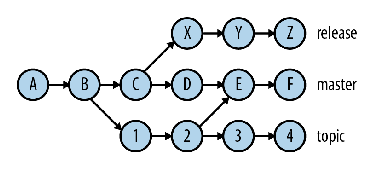
\includegraphics[width=0.3\columnwidth]{gitgraph}
	\caption{Exemple d'arbre de commits Git}
	\label{fig:git}
\end{figure}
\subsection{Bilan}

%%%%%%% SECTION %%%%%%%
%\section{Architecture de communication hybride}

%%%%%%% SECTION %%%%%%%
\section{Architecture de communication hybride}

%\subsection{Introduction}

Dans la section précédente, l'introduction du modèle orienté événements 
s'intéresse principalement à ce qui se passe au sein d'un seul client. 
Or la collaboration passe par la mise en relation des différents collaborateurs, mais aussi par  
l'échange des données nécessaires à la collaboration (données de connexion, 
mises à jour de la scène, sensibilisation\dots)
Afin de pouvoir proposer un \gls{SEC} adapté aux besoins de l'édition de scènes 
3D, plusieurs types de granularité sont à distinguer : 
\begin{itemize}
	\item une granularité fine pour l'édition massive ;
	\item une granularité liée aux spécificités de la modélisation \gls{3D} ;
	\item et une granularité reposant sur des technologies web (réseau, interface, 
	interaction \gls{3D}).
\end{itemize}

Les systèmes \gls{P2P} qui sont orientés événements consistent en plusieurs 
n\oe uds interconnectés dont les fonctions et l'exécution des tâches sont
similaires. Les pairs partagent directement leurs ressources (contenu, CPU, 
stockage, bande passante) sans nécessiter de serveur central. A la place, les 
pairs coopèrent au moyen d'événements qui prennent la forme de messages lorsqu'ils
se les échangent. Les systèmes \gls{P2P} sont capables de s'adapter aux 
dysfonctionnements et à la dynamicité des pairs, tout en maintenant des 
performances acceptables. Les systèmes \gls{P2P} sont généralement utilisés 
comme soutien aux services de l'application pour la communication et la 
collaboration, le calcul distribué, la distribution de contenus et pour les services 
d'intergiciel comme le routage et la localisation, ou encore l'anonymat et la confidentialité.

\paragraph{Constat} Les \glspl{SEC} ont connu un fort développement avec 
l'intérêt 
croissant 
pour le \gls{P2P} dans les années 2000. 
La base théorique des \glspl{SEC} s'appuie sur les propriétés de 
convergence, préservation de la causalité et préservation de l'intention du modèle 
\acrshort{CCI} \cite{Sun1998}. 
La plupart des travaux liés aux \glspl{SEC} \gls{P2P} s'intéressent à 
l'édition collaborative massive de documents textuels dont les propriétés 
de commutativité sont plus faciles à gérer (insertion / suppression) en 
comparaison à celles concernant la \gls{3D} (multiplication de matrices de 
rotation). La génération de conflits en \gls{3D} peut vite devenir incontrôlable. Il est 
donc nécessaire de mettre en place des mécanismes de détection de 
conflits et de maintenir une cohérence au cours des sessions de 
collaboration. 





%\gls{WebRTC} est une technologie qui fournit aux navigateurs 
%\textit{destkop} et mobiles la possibilité de communiquer en temps-réel 
%(cf \ref{sec:webrtc} via une collection de standards, 
%protocoles et \glspl{API} JavaScript. 
%L'un des atouts de cette technologie est de permettre de façon simple et 
%sans module d'extension la capture d'un flux audio et / ou vidéo (ex : 
%applications de VoIP), ainsi que l'échange de données arbitraires entre 
%navigateurs sans nécessiter d'intermédiaires (ex : partage de fichiers en 
%\gls{P2P}).
%Techniquement, \gls{WebRTC} supporte un canal temps-réel 
%bidirectionnel pour l'échange de données. Contrairement à 
%\gls{WebSocket}, qui est basé sur \gls{TCP}, \gls{WebRTC} repose sur 
%\acrshort{UDP} en intégrant une pile de plusieurs protocoles (Figure 
%\ref{fig:protocolstack}) qui lui offre des fonctionnalités similaires (fiabilité, 
%ordonnancement, sécurité). 

%TODO parler chargeet distribution


\paragraph{Contribution}
La mise en place d'une architecture de communication 
hybride permet de concilier à la 
fois les avantages d'une architecture client-serveur et ceux du \gls{P2P}, en évitant 
certains désavantages occasionnés dans ces derniers (engorgement du serveur, 
pair seul sur le réseau\dots). 
Le terme \og hybride\fg{} invoque un compromis entre la 
centralisation de l'information nécessaire à la prise de décision globale et 
la décentralisation des échanges utile à l'amélioration du partage de 
contenus \gls{3D} à l'échelle locale. 
En agissant sur ces deux échelles, la granularité de la collaboration est plus fine. 
Par exemple, le passage à l'échelle est facilité par la présence de 
ressources locales et la coordination des utilisateurs se fait à une échelle 
globale, ce qui permet également l'accès à une source de vérité 
centralisée (base de données) et commune.
Dans le contexte des \glspl{EVC3D}, le but 
est d'obtenir une architecture de communication : 

\begin{itemize}
	\item entièrement basée web ; 
	\item robuste face à l'évolution du nombre de collaborateurs ; 
	\item efficace en termes d'accès et de distribution de la donnée ; 
	\item et qui s'adapte à l'échelle selon les besoins de la collaboration.
\end{itemize}


Tous les travaux liés à cette thèse 
\cite{Desprat2015a,Desprat2015b,Desprat2016,Desprat2017} s'appuient sur une 
architecture de communication hybride tripartite (Figure \ref{fig:hybrid}) pour 
faire de la modélisation \gls{3D} collaborative : serveur, persistance 
et les pairs\footnote{Les pairs sont appelés \og Clients\fg{} dans les premiers 
travaux}. 

Les contributions portées par Desprat et al. dans \cite{Desprat2015a} et \cite{Desprat2015b} 
s'appuient sur des pairs ayant un rôle simple et proposent une transmission des 
mises à jour en tant que différentiel d'état. Les conflits lors d'opérations 
concurrentes sont évités grâce à un mécanisme de verrouillage. 
Plus tard, dans \cite{Desprat2016}, les auteurs mettent en place le modèle 
orienté événements qui impose l'évolution, au niveau réseau, du protocole 
de transmission (celui-ci reposant sur 
des notifications d'événements et la gestion des flux d'agrégat). 
Plus récemment, dans \cite{Desprat2017}, est apparue la distinction entre 
les deux rôles parmi les pairs : la 
partie serveur se compose désormais de pairs qui ont un rôle de vérification 
de la cohérence et de relais des données dans la couche \gls{P2P}. Cette 
contribution intervient dans le but d'encourager la résilience du système et la 
vitesse de dissémination des informations dans le réseau, en favorisant la prompte 
détection de conflits (source de vérité plus proche des pairs producteurs). 
Cette extension repose sur la présence d'un journal d'événements partagé et 
répliqué sur les pairs participants à la collaboration.

\begin{figure}[h!]
	\centering
	\includegraphics[width=0.7\columnwidth]{eps/hybrid5.eps}
	\caption{Architecture hybride tripartite : serveur, persistance 
		et les pairs.}
	\label{fig:hybrid}
\end{figure}

Cette section décrit le modèle d'architecture mis en 
place pour gérer la transmission de contenu entre les différents clients 
qui participent à l'édition collaborative d'un espace de travail \gls{3D} partagé. 
Les différents protocoles de transmission, issus des travaux sus-nommés, 
sont présentés. Ils montrent ainsi l'évolution de l'architecture de communication de 
sa version naïve à la version étendue, plus proche des considérations métiers et 
offrant plus de liberté dans la création grâce la mise en place d'un système inspiré 
des \glspl{CRDT}.
 
Les différents éléments constitutifs d'un pair sont détaillés avant la présentation 
des deux types de pairs rencontrés dans l'architecture.
Sont expliqués ensuite les mécanismes de mise en relation de 
ces composants pour que les différents participants d'une session 
collaborative puissent communiquer de manière transparente, cohérente et 
résiliente.

%TODO reprendre pour partie implantation
%Les travaux présentés s'inscrivent dans un contexte où les besoins 
%d'interopérabilité et de standardisation sont élevés pour permettre à des 
%utilisateurs de prendre le système rapidement en main sans installer autre chose 
%qu'un navigateur. 


\subsection{Éléments constitutifs d'un pair}
Dans un réseau \gls{P2P}, chaque pair est considéré comme un système à part 
entière qui contient ses propres problématiques d'implémentation. Avant de 
présenter la contribution liée à l'intergiciel dans 3DEvent, il est nécessaire 
d'introduire les composants et les fonctions clés qui constituent un pair du point de 
vue strictement réseau en 
présentant une vue minimaliste d'un pair dédié au partage de contenu 
\cite[p.135-136]{Buford2009}. Les 
fonctions sont divisées en trois :
\begin{itemize}
	\item la couche de routage et d'échange de messages ;
	\item la recherche et le stockage de contenu ;
	\item ainsi que la configuration et sélection du rôle du pair.
\end{itemize}


\begin{figure}[ht]
	\centering
	\inputTikZ{0.9}{eps/tikz/middleware/middleware}
	\caption{Composants de chaque pair dans 3DEvent (point de vue réseau)}
	\label{fig:middleware}
\end{figure}


Chaque pair générique fournit de base une \gls{API} pour les fonctions d'échange 
de messages et de recherche. 
L'\gls{API} de recherche est principalement en lien avec le 
gestionnaire d'instances qui se charge de la recherche, mais il est possible de se 
connecter à des pairs via d'autres pairs si le serveur est absent ou pour renforcer 
le maillage.
L'élément responsable de la couche de routage et d'échange de messages permet 
à chaque pair de maintenir un état de connexion avec ses voisins dans la couche 
; maintenir cet état inclut la découverte de voisins et la maintenance  à jour des 
états des voisins.
Un pair possède un mécanisme d'amorçage (\textit{bootstrap}) qui permet de 
localiser les autres pairs qui lui permettront de rejoindre la couche \gls{P2P}. Les 
étapes pour rejoindre ou quitter la couche sont proposées par le protocole 
d'établissement de connexion 
(cf signaling mecanism\todo{ref section signaling}).
La couche applicative permet  d'échanger des messages avec les autres pairs 
dans le réseau en utilisant l'\gls{API} réseau, et les messages reçus peuvent être 
transférés à leur destination en utilisant la fonction de transfert de messages. 

Le contenu partagé est stocké localement pour pouvoir être accessible par d'autres 
pairs, ainsi que l'interface de l'application du pair courant. Le contenu doit être 
organisé pour la recherche d'informations afin de fournir une indexation et une 
interface de requête. 
L'espace de stockage pour les données partagées va correspondre aux différents 
états des agrégats \cite{Desprat2015a,Desprat2015b} ou au journal d'événements 
\cite{Desprat2016,Desprat2017}.


La dernière fonction concerne la manière dont le pair auto-organise, à la fois, ses 
ressources locales et son rôle dans le réseau. Le pair détermine les 
ressources du système et du réseau disponibles et peut surveiller les 
changements éventuels régulièrement.
Le pair a connaissance du rôle qui lui est attribué à sa création dans le réseau. Les 
rôles des pairs (super pair, relai, producteur\dots) dépendent de 
capacités comme les ressources du système et du réseau. Le rôle induit les 
capacités et la configuration de chaque pair, i.e. un pair actif est configuré 
uniquement pour produire, stocker et relayer les données tandis qu'un pair passif ne fait que stocker et relayer les données. La stabilité du pair peut être indiquée par son niveau de 
\textit{churn} (dynamicité : rejoindre et quitter un réseau) par exemple. 
La Figure \ref{fig:middleware} peut être affinée en fonction du type de 
réseaux et d'applications. Chaque pair comprend un protocole pour la gestion
de sessions (ex: REST API) et pour l'échange de données (ex: RTCDataChannels)  
pour pouvoir participer à la collaboration.



Les architectures de communication des contributions se divisent en deux parties, 
chacune correspondant au paradigme qu'elles utilisent respectivement : état ou 
événement. Selon le paradigme auquel elles font référence, elles peuvent 
être décrites par plusieurs critères:
\todo{revoir}
\begin{description}
	\item[Spécificité des composants de l'architecture] Les pairs sont la base de la 
	dissémination de l'information. La partie serveur 
	centralise les données liées à la persistance long  terme et
	décentralise la réplication des données à court terme. Cela évite au 
	serveur 
	d'être le point central des échanges en déchargeant les canaux passant par le 
	serveur.
	\item [Gestion de la session] 
	La gestion de la session suit le cycle de vie des pairs au sein du réseau 
	lorsqu'ils participent à une session collaborative. 
	Pour intégrer le réseau \gls{P2P} et participer à l'édition d'une scène \gls{3D} de 
	manière collaborative, les clients passent par les étapes suivantes :
		\begin{enumerate}
		\item Phase de \textit{signaling}
		\label{phase1signaling}
		\begin{enumerate}
			\item Signification de la présence auprès du serveur de \textit{signaling}
			\item Récupération de la liste des identifiants des pairs auxquels se 
			connecter
			\item Création d'une connexion \gls{P2P} avec les autres pairs
			\item Souscription aux flux
			
		\end{enumerate}
		\item Phase de synchronisation
		\label{phase2sync}
		\begin{enumerate}
			\item Requête des données manquantes
			\item Récupération des données manquantes
			\item Ré-ordonnancement des messages reçus
			\item Maintien de la cohérence (détection de conflit)
		\end{enumerate}
		
		\item Phase de génération de nouvelles données valides 
		\label{phase3gen}
		\begin{enumerate}
			\item Publication des données aux voisins
		\end{enumerate}
		
		\item Phase d'abandon
		\label{phase4quit}
		\begin{enumerate}
			\item Notification aux voisins 
			\item Fermeture des canaux
		\end{enumerate}
	\end{enumerate}
	
	Ces quatre phases sont distinctes même si, lorsqu'un pair initialise ou rejoint 
	une 
	session collaborative (séquence d'initialisation), les phases 
	\ref{phase1signaling}, \ref{phase2sync} et \ref{phase3gen} s'enchainent pour 
	ce pair. Durant la session collaborative, les phases \ref{phase2sync} et 
	\ref{phase3gen} s'alternent. La phase \ref{phase4quit} se produit lorsque qu'un 
	client quitte une scène de manière volontaire (changement de scène, fermeture 
	de l'onglet du navigateur) ou involontaire (fausse manipulation, navigateur en 
	panne, coupure internet) signifiant la fin de la session collaborative.
	
	\item [Gestion du stockage et structure des données] 
	Le stockage peut prendre plusieurs formes : \textit{in-memory}, stockage local, 
	disque dur\dots selon le type de stockage adapté et disponible. 
	Dans l'architecture hybride, il existe deux niveaux de stockage : la persistence 
	long-terme, distante -- la base de données -- et la persistence court-terme, 
	locale -- le navigateur.
	Le serveur assure, d'une part, la centralisation du stockage à long-terme, et 
	d'autre part, la mise en relation des différents clients.
	\item [Gestion de la synchronisation et de la cohérence (détection des conflits)] 
	Il existe différentes possibilités de synchronisation des pairs. 
	
	L'édition concurrente lors de la collaboration peut être gérée de différentes 
	manières, selon si elle est plutôt pessimiste ou optimiste lors de la réplication 
	des 
	données (voir Section \ref{sec:concurrence}). L'intégration d'une solution ou 
	l'autre 
	a de lourds impacts sur l'expérience utilisateur (fonctionnalités, interface 
	utilisateur) et la gestion de la cohérence dans le réseau \gls{P2P}.  
	
	\item [Protocole d'échange]
	La couche \gls{P2P} fournit une dissémination rapide de l'information et 
	\todo{finir}
\end{description}


%
%\subsection{Architecture de communication \og orientée états\fg{}}
%\label{sec:comm_state}

\subsection{Architecture hybride \og orientée états\fg{}}
\label{sec:comm_state}

Les premiers travaux liés à cette thèse \cite{Desprat2015a,Desprat2015b} se sont 
intéressés principalement à la mise en place de l'architecture de communication 
en basant les structures de données sur des états (plutôt que des événements). 
Cette section décrit les choix faits lors de la modélisation de l'architecture \og 
orientée état\fg{}, pour le stockage et le transfert par exemple, en lien fort avec les 
technologies web sous-jacentes.  
%l'architecture est principalement s'app
%The client-server part is based on a REST (Representa- tional State Transfer) 
%architecture [TV10] that benefits from distributed hypermedia systems such as 
%our. 
%
%
%Pros
%Easier to maintain
%No need to keep a permanent an open connection
%Web context: use of HTTP protocol, URI as resource representative, server 
%caching
%
%
%Cons
%Bandwidth increasing and latency: client needs to keep locally all the necessary 
%data to send the request
%  Table 1 resumes the advantages and the drawbacks of a RESTful system. It 
%fits 
%  well for web distributed sys- tems even if mobile devices should have limited 
%  perfor- mance due to back and forth requests that are energy consuming.
%  
\subsubsection{Spécificité des composants de l'architecture}
Le système présenté repose sur une architecture \acrshort{REST} 
(\acrlong{REST}) concernant les échanges clients-serveur. Cette architecture 
permet de séparer les responsabilités entre le client et le serveur en séparant 
l'\gls{IU} du stockage. \gls{REST} propose une interface uniforme. Cela implique 
que chaque ressource est identifiée et manipulable par des représentations définies 
(modification, suppression). 

Chaque pair correspond a un client (navigateur web) qui contient l'intergiciel 
\gls{P2P} offrant des fonctionnalités limitées, l'interface utilisateur contenant 
l'environnement \gls{3D} et un espace de stockage reposant local (IndexedDB).

La persistance long terme est une base de données NoSQL. Ce type de bases de 
données a tendance à être optimisée en lecture (grâce à un 
langage de requête dédié) et permet d'éviter les 
structures rigides. Cette flexibilité est utile lors du stockage des modèles \gls{3D} 
et 
encourage la conservation d'autres métadonnées (ex: relations entre les différents 
objets) pour faciliter la traçabilité. 
Avec une base de données centralisée, le système possède une source de 
données fiable et autoritaire qui permet à un utilisateur de récupérer le bon contenu 
quand il revient sur une scène. La totalité du document, contenant la scène, est 
envoyé à l'utilisateur lorsqu'il y accède.


\subsubsection{Gestion du stockage et structure de données}

Avec une base de données NoSQL utilisant des schémas dynamiques, les 
données sont stockées sous forme de document. Chaque document est 
auto-descriptif et peut contenir des valeurs qui s'imbriquent sous la forme d'une 
structure en arbre hiérarchique. Une collection consiste à grouper des documents, 
équivalent dans une base de données relationnelle à la notion de table. La base de 
données contient deux types de collections : les scènes et les géométries. Une 
collection de scènes contient des scènes qui sont décrites par leur identifiant et 
les méta-données de l'espace virtuel \gls{3D}, ainsi que la liste des contributeurs et 
la 
liste des maillages. Cette liste correspond à une association entre un identifiant de 
maillage, les méta-données de l'objet et l'identifiant d'une géométrie existante. 
Les géométries sont, quant à elles, stockées avec leur identifiant propre et l'objet 
3D complet donné sous le format \gls{JSON}.

Sur chaque pair, il existe un stockage relationnel (IndexedDB) pour 
chaque objet de la base de donnée récupérée. Cela permet au client de faire des 
requêtes directement dans son espace local si besoin, par exemple en ajoutant un maillage. 
C'est également une source pour transférer ses modifications aux autres clients.
Les navigateurs permettent désormais de stocker des quantités de données 
importantes localement avec une durée de vie illimitée. 
Les paramètres des opérations fondamentales effectuées sur la base de données 
(\gls{CRUD}) sur les collections sont très bien supportés par les requêtes 
\gls{REST}.


\subsubsection{Gestion de la session}
Lorsqu'un utilisateur rejoint une session, il suit le déroulement des opérations 
décrit dans la Figure \ref{fig:sequence_state}. 
Dans un premier temps, afin de récupérer les données liées à l'espace de travail, 
le client web de l'utilisateur qui se rend sur une scène récupère 
tous les objets associés à la scène dans la base de données. Les objets de la 
scène sont renvoyés à l'éditeur pour les afficher. 
Dans un second temps, le système établit les connexions \gls{P2P} entre les 
clients de manière automatique et complète (topologie réseau en maillage 
complet) après avoir récupéré les identifiants des autres utilisateurs auprès du 
serveur de \textit{signaling}. Une fois la connexion établie, chaque collaborateur 
voit son environnement \gls{3D} dans l'éditeur mis à jour, indiquant la position du 
nouvel 
arrivant. Les collaborateurs éditent ensuite la scène \gls{3D} qui produit, sur les 
différents objets, des requêtes \gls{CRUD} -- incluant les opérations de translation, 
rotation et homothétie -- destinées au serveur (qui transmet les 
modifications à la base de données) puis aux collaborateurs.
Enfin, dans un dernier temps, lorsque l'utilisateur quitte la scène, il en notifie le 
serveur de \textit{signaling} qui s'occupe d'indiquer aux clients restants l'abandon 
du client pour qu'ils puissent mettre à jour leur interface en conséquence.

\begin{figure}[ht!]
	\centering
	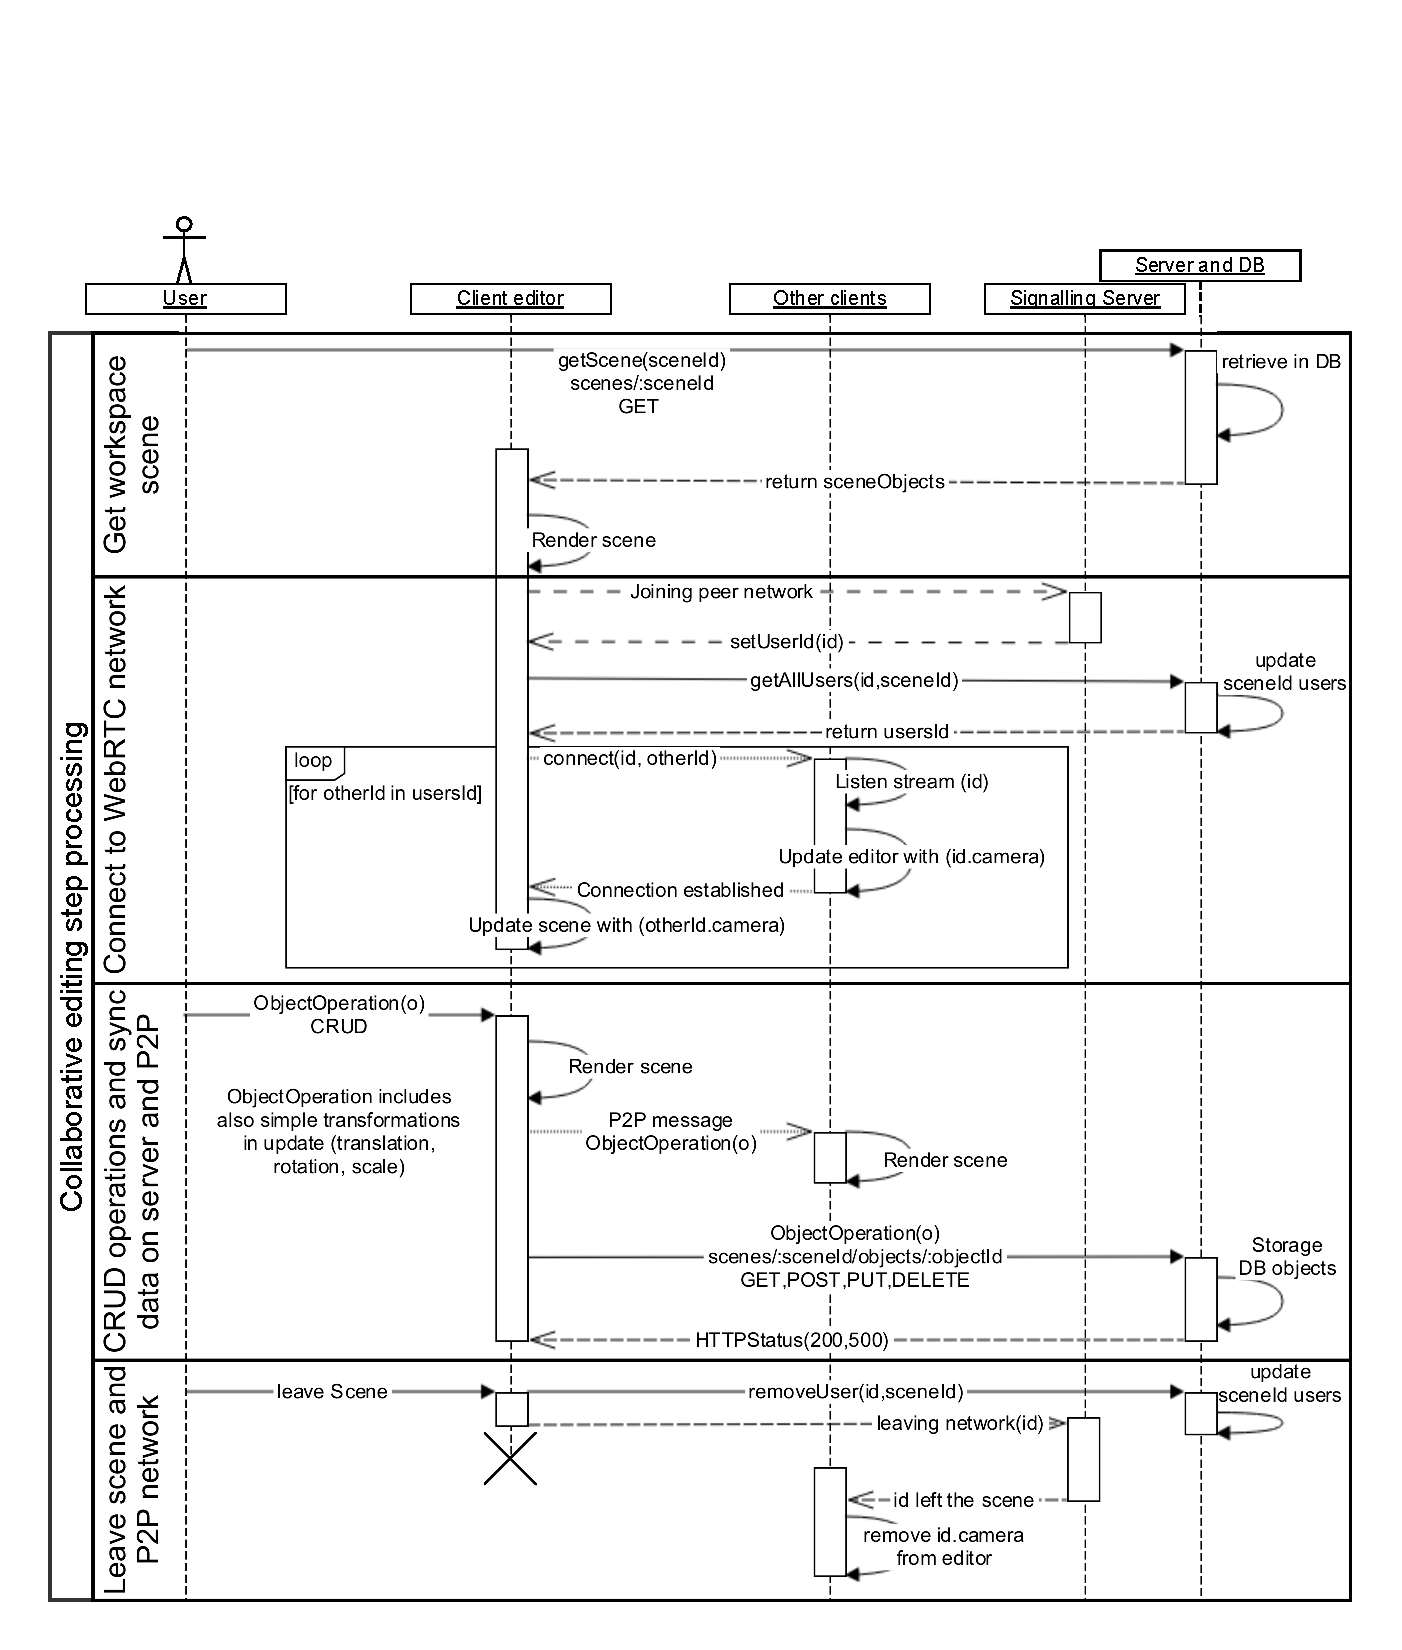
\includegraphics[trim={0 0 0 3cm},clip,width=1\columnwidth]
	{eps/sequence_wscg.eps}
	\caption{Diagramme de séquence de la gestion de la session dans une 
	architecture \og orientée état\fg{}}
	\label{fig:sequence_state}
\end{figure}

%
%We propose to auto connect users on a scene with a We- bRTC connection. As 
%each user send their ID to the database at their arrival, they also retrieve those 
%which where already present on the scene. We are able to cre- ate a full mesh 
%topology network in order to make them communicate the updates.
%
%Even if we have a full mesh topology, the P2P message layer is more similar 
%the 
%star topology. Indeed, the Fig- ure 2 shows the path of a sent message 
%operation 
%on the connection and it is only sent to the one degree neigh- bors of the original 
%broadcaster (the “B” node on the Figure 2).
%
%
%We choose to keep reliable and in order delivery for now. The RTCDataChannel 
%API supports many data types (strings, binary types: Blob, ArrayBuffer. . . ). 
%These types are helpful in a 3D multi user environment to broadcast messages 
%including the objets and their transformations. We tried to limit the amount of 
%data 
%by sending only relevant information but there is actually no particular 
%optimization. The channel can be over- feed when an object is imported then 
%pushed through the network.
%

\subsubsection{Gestion de la synchronisation et de la cohérence}
\label{sec:synchronisation-client-serveur}

Les travaux \cite{Desprat2015a} et \cite{Desprat2015b} présentent une version 
naïve du processus de synchronisation. La cohérence est garantie par un système 
de verrouillage des objets. Cela évite notamment les sélections concurrentes et par 
conséquent les éditions concurrentes. 
Lors de la récupération de la scène, elle est considérée comme cohérente. 
Ensuite, le choix d'avoir des connexions \gls{P2P} ordonnées et fiables, ainsi qu'un 
maillage de pair complet, implique que toute donnée envoyée par un pair est 
forcément reçue par les autres. 

Lors de la connexion d'un nouveau client, a lieu la synchronisation des deux 
systèmes de persistance pour obtenir les mises à jour : 
\improve{l'échange des mises à jour entre le client (persistance à court terme) et la 
	base de données (à long terme) afin de synchroniser les deux éléments avec. 
	La base de données peut également servir en cas de conflits importants ; elle sert 
	de référent.}
\begin{enumerate}
	\item depuis le client, où l'on distingue trois cas :
	\begin{enumerate}
		\item travail "\textit{offline}" (hors ligne) : l'utilisateur a travaillé hors ligne et 
		doit maintenant publier "en ligne" son travail. Les mises à jour sont publiées sur la 
		base de données ; le serveur vérifie si aucun conflit ne survient puis 
		fusionne (\textit{merge}) les nouvelles entrées avec l'existant; 
		
		\item travail "\textit{serverless}" (en collaboration avec entre pairs sans le 
		serveur) : dans le cas où le serveur est absent, les clients peuvent continuer 
		de créer en collaborant. Ces données n'étant stockées que sur le client, il est 
		nécessaire de les transmettre à la base de données dès qu'une connexion 
		est possible. 
		Cela peut être fait en une fois ou de manière partagée\improve{ça veut dire 
			quoi?};
		
		\item travail "\textit{online}" (en collaboration entre pairs comprenant la partie
		serveur) : le client envoie régulièrement \improve{combien de temps} ses 
		nouvelles modifications pour qu'elles soient intégrées à la base de données.
	\end{enumerate}
	\item depuis la base de données :
	Le client reçoit toutes les nouvelles mises à jour de la scène depuis la dernière 
	fois qu'il s'est connecté. Cela peut également inclure des mises à jour qui sont 
	en conflit avec ce qu'il y a dans son propre espace de stockage, qu'il lui faut 
	donc modifier.
	Dans le cas où un utilisateur est seul connecté, la base de données est la 
	seule source disponible pour la mise à jour du client. 
\end{enumerate}


Le fait de synchroniser un client avec une base de données NoSQL dès que cela 
est possible permet de supporter les connexions intermittentes comme pour les 
appareils mobiles dans cette architecture ; cette approche est connue sous le nom 
de \og\textit{offline first}\fg{} \cite{Gadea2016}.
\subsubsection{Topologie et protocole d'échange}
Cette architecture est basée sur une topologie de maillage complet (\textit{full 
mesh topology}) pour le réseau \gls{P2P}.
Les échanges se font donc à deux niveaux: entre les pairs, ainsi qu'entre chaque 
pair et la base de données. Pour le premier niveau, la couche réseau \gls{P2P} est 
assez 
naïve dans le sens où les connexions sont considérées comme fiables et 
ordonnées ; le client n'a alors qu'à publier toutes les modifications qu'il effectue et 
les envoyer à tous les clients (auxquels il est nécessairement connecté).
Les pairs échangent des différentiels d'état sur les objets. Ces messages ne 
contiennent pas d'information sémantique sur le type d'action effectuée par chaque 
utilisateur. 

\subsubsection{Discussion des problématiques liées à une architecture de 
communication orientée \og états\fg{}}

La base de données centralisée est beaucoup sollicitée lors des sessions 
collaboratives, ce qui peut mener à une surcharge similaire aux architectures 
uniquement client-serveur. 
En combinant client-serveur et \gls{P2P}, la charge aurait dû être réduite et 
transférée aux autres pairs, notamment lors de la phase de récupération d'une 
nouvelle scène qui repose entièrement sur le serveur. 
Chaque pair assume la responsabilité dans l'envoi de ses modifications à tous les 
autres pairs. Cette tâche ne profite pas du réseau \gls{P2P} de manière optimale 
car la topologie ne profite pas de la fonction relais des pairs. Cela pourrait alléger  la 
distribution dans la couche \gls{P2P} et responsabiliser un peu plus les pairs pour 
faciliter le passage à l'échelle.
En effet, la topologie en maillage complet limite le passage à l'échelle car le 
nombre de connexions va croître de manière exponentielle. 

Par ailleurs, les requêtes \gls{CRUD} ne sont pas très expressives concernant le 
métier. 
Aucune vérification n'est donc effectuée sur la validité des données transmises 
dans cette architecture. De plus, il peut arriver, du fait de latences réseaux que les 
modifications des différents utilisateurs s'entrelacent à l'arrivée et ne rendent pas 
l'intention de l'utilisateur. Cela peut mener à des dé-synchronisations fortes.

Concernant la gestion de la concurrence, l'utilisation d'une solution pessimiste 
dans un environnement \gls{P2P} peut parfois mener à des inter-blocages si un 
utilisateur quitte la scène sans avoir relâché l'objet, c'est à dire sans en avoir 
informé la base de données et les autres 
utilisateurs. 
Même si l'application peut prendre le relais et permettre la relâche du 
verrou au bout d'un certain temps, l'expérience utilisateur peut être dégradée 
pendant cette période.
Le maintien de la cohérence est a peu près garanti dans ce modèle si l'on 
considère un environnement où la fréquence des modifications n'est pas très 
élevée, et que tous les clients communiquent leur horloge locale pour établir un 
référentiel de temps concernant les mises à jour. 

Enfin, le transfert par différentiel d'état utilisé pour réduire la taille des 
données liées au changement d'état des objets lors de la transmission des 
données peut varier grandement selon le type de changement 
effectué, rendant peu prévisible la charge des canaux de communication. 
%
%Some issues remain in RTCDataChannel API : the com- patibility and 
%interoperability is still not complete be- tween browsers6, some browsers (like 
%Chrome) im- pose a send limit (about 6MB) for the data transmitting through 
%DataConnections and the security of the com- munication is still vulnerable7. 
%The 
%system overview (Figure 4) illustrates the communication architecture topology 
%between the peer clients and server (plus sig- naling).



%\subsection{De l'état à l'événement}
%\label{sec:statetoevent}

\subsection{De l'état à l'événement}
\label{sec:statetoevent}
Afin d'intégrer la notion d'historique dans une application web, plusieurs indicateurs 
sont nécessaires (version, granularité de l'historisation, type et taille des données 
manipulées). Cette section décrit le processus pour passer d'un système basé 
états à un système basé événements dans l'intérêt de réduire la somme des 
données transmises sans perdre d'information concernant la logique métier.
\paragraph{Description des variables}
Une scène $S$ contient l'ensemble des $n$ objets $x$ ($S =\{x_0,x_1,...,x_n\}$). 
Chaque élément de $S$ est associé à une taille calculée comme la somme des 
modifications $m$ selon la version $v$. 

Pour tout objet $x$ appartenant à la scène $S$ on associe une taille $w \in 
\mathbb{R}$. $w$ correspond à la taille totale des données transmises pour 
modifier l'objet à chaque version $v$ ($v$=0 correspond à la taille de l'objet à l'état 
original, i.e. l'\gls{EventStore} est vide). La taille totale de la scène, notée $Sw$, 
correspond à sommer la taille de tous ses objets (équation \ref{eq:sw}). Toutes les 
variables évoquées sont exprimées en octet pour avoir des termes avec des 
unités homogènes.

\begin{equation}
\label{eq:sw}
\text{Taille d'une scène $S$ : } S_w= \sum_{i=0}^{n}w_i
\end{equation}


\paragraph{Transmission par état}
Dans un système où à chaque modification on transmet l'état complet (équation 
\ref{eq:complet}), la taille des éléments transmis correspond à la somme de tous 
les états par lesquels l'objet est passé. Cette valeur va augmenter par paliers de 
tailles du même ordre de grandeur.
La transmission par état propose un historique issu d'une sauvegarde 
chronologique. Cependant elle est lourde voire redondante et n'offre pas 
d'information sur l'intention de l'utilisateur (quelle opération a permis d'arriver à cet 
état?).

\begin{equation}
\label{eq:complet}
\text{Par état : } w_i = \sum_{v=0}^{n}state_{v}
\end{equation}


\paragraph{Transmission par différentiel d'état}
\label{par:diff}
Dans un système où l'on transmet un différentiel d'état (équation 
\ref{eq:différentiel}), la différence entre deux états peut être difficile à exprimer (ex: 
MeshHisto \cite{Salvati2015})
car il s'agit d'un objet 3D dont les informations, stockées dans 
un fichier, ne sont pas linéaires. Le différentiel peut beaucoup varier jusqu'à 
atteindre une taille proche de l'état actuel si une transformation génère beaucoup 
de modifications par rapport à l'état précédent. A contrario, une modification sur la 
position d'un objet peut être très légère. La fonction représentant la taille des 
ressources transmises augmentera par palier avec au pire les propriétés de la 
proposition précédente (équation \ref{eq:complet}). Le différentiel d'état permet 
d'alléger la transmission par rapport à la proposition précédente, ne contenant 
cependant pas d'information sémantique sur ce qui est transmis et les opérations 
qui ont conduit à l'état d'un objet 3D de la scène.

\begin{equation}
\label{eq:différentiel}
\text{Par différentiel d'état : } w_i = state_0 + \sum_{v=1}^{n}(\underbrace{state_{v} 
- state_{v-1}}_{differential})
\end{equation}

\paragraph{Transmission par événement}
La transmission par événement (équation \ref{eq:evenement}) repose sur le 
principe du différentiel d'état ($differential$) exprimé ci-dessus (équation 
\ref{eq:différentiel}) en ajoutant la notion de type d'événement ($eventType$). Le 
type d'un événement indique le nom de la transformation à appliquer pour passer 
d'un état à l'autre. Un événement contient par nature une sémantique <<métier>> 
associée à chaque opération qui donne des indications sur l'intention de 
l'utilisateur. 

\begin{equation}
\label{eq:evenement}
\text{Par évènement : } w_i= state_0 + \sum_{v=1}^{n}(\underbrace{eventType + 
differential}_{event}) 
\end{equation}

Dans un \gls{EVC3D}, il y a des événements concernant à la fois la manipulation 
3D, la navigation et les éléments se rapportant à la collaboration (par exemple: 
prendre le point de vue d'un collaborateur). La taille d'un événement est variable 
(comme un différentiel d'état) avec un minimum contenant le type d'événement 
($eventType$) dû à sa structure type/paramètres. Cette proposition est un peu 
plus lourde à transmettre que la précédente mais ajoute une valeur sémantique à 
l'historique.



%\subsection{Architecture de communication \og orientée événements\fg{}}
%\label{sec:comm_event}

\subsection{Architecture de hybride \og orientée événements\fg{}}
\label{sec:comm_event}



\subsubsection{Persistance à long terme}\label{sec:persistance-a-long-terme}
Dans un contexte industriel de collaboration, l'information doit être disponible sur le 
long terme, facilement accessible par l'entreprise. La persistance à 
long-terme stocke le journal d'événement qui est la 
source de vérité de l'application. Elle peut également stocker des projections 
prédéfinies, calculées à la volée ou encore des \textit{snapshots} de l'application.



\subsubsection{Mécanisme de gestion de version}
3DEvent intègre une procédure de gestion de version dans l'\gls{EventStore} afin 
de gérer au mieux la cohérence des données. 
Chaque gestion de commande (Figure \ref{fig:gestionCommande}) entraîne la 
génération d'un ou plusieurs événements. Ces événements sont considérés 
comme \og soumis\fg{} (\textit{uncommitted}) mais pas encore <<~publiés~>> 
(\textit{committed}).  Pour qu'ils le deviennent, l'agrégat concerné par ces 
événements doit produire une nouvelle version sans être en conflit avec la 
précédente. En passant la version attendue $v_a$ au gestionnaire de conflit, on 
est à même de la comparer avec la version courante $v_c$. Il existe deux cas où 
un conflit est levé~: 
\begin{enumerate}[label=\alph*)]
	\item \label{i:vi} La version $v_a$ correspond à la valeur d'initialisation
	\item \label{i:vdiff} La version $v_a$ est différente de la version $v_c$
\end{enumerate}
Dans \ref{i:vi}, on s'assure qu'après une action la version initiale de l'agrégat ne 
peut être la même. Cet item peut sembler évident mais il est important de le noter 
car il dépend entièrement de la valeur initiale choisie pour les agrégats du 
\gls{framework} (on peut commencer à n'importe quelle valeur -- -1, 0\ldots).


%
%\subsubsection{Gestion de la cohérence}
%
%
%\subsubsection{Respect de la causalité}
%\subsubsection{Convergence des répliques}
%\subsubsection{Préservation de l'intention}
\subsubsection{Extension : Event Store distribué}


%\paragraph{Connexion des pairs en début de session}
Dans \cite{Desprat2017}, lorsqu'un pair initialise ou rejoint, la séquence pour 
rejoindre une session collaborative évolue 
pour prendre en considération l'intégration des événements et la synchronisation 
des journaux d'événements.
La Figure \ref{fig:connexionpairs} représente la séquence d'actions nécessaire à 
une instance 3DEvent ($idA$) pour rejoindre le réseau contenant déjà d'autres 
instances 3DEvent. L'action \textit{join} est exécutée lorsqu'un utilisateur envoie 
ses informations de connexion sur un portail de connexion (à partir d'une instance 
web) ou lorsqu'une instance serveur est lancée. Cette action ajoute le nouveau 
pair à la liste des pairs présents sur le réseau. La liste est gérée par le 
gestionnaire 
d'instance, et retourne la liste des pairs avec lesquels le pair doit se connecter. 
Pour chaque pair $idB$ de la liste retournée $ids$, $idA$ utilise le mécanisme de 
signalisation (offre/demande). Le mécanisme est déclenché par l'instanciation d'un 
\textit{network bridge}\info{definir} dans l'\textit{event store} \info{definir} de $idA$ 
puis celui de $idB$. Afin de resynchroniser les deux pairs (après cette série 
d'échanges asynchrones), $idA$ et $idB$ s'échangent des métadonnées sur la 
situation respective de leurs \textit{ESM} \info{definir} afin de se synchroniser 
\info{(see refernece sync mechanism}.

\begin{figure}[h]
	\noindent
	\centering
	\includegraphics[width=\columnwidth]{connection.eps}
	\caption{Protocole de connexion au réseau d'instance 3DEvent}
	\label{fig:connexionpairs}
\end{figure}



L'Event Store est un composant clé dans le traitement des événements. Il prend 
en entrée des événements générés ou reçus extérieurement et produit en sortie 
des événements cohérents qui peuvent être par la suite publiés. Les événements 
sont considérés comme cohérents lorsqu'il n'y a pas d'erreur de cohérence, i.e. 
lorsque les numéros de versions sont bien ordonnés. Chaque Event Store contient 
deux éléments: l'Event Stream Manager (ESM) et des Network Bridges (NB). Un
ESM est une structure de données représentée par une collection de flux 
d'événements. Un flux d'événement est représenté par un tableau d'événements 
indexés en séquence permettant de stocker les événements d'un aggrégat dans 
l'ordre temporel. Si un flux ne rencontre pas de problème de cohérence alors le 
dernier index correspond au numéro de version de l'agrégat. Lorsque l'Event Store 
reçoit un événement de l'instance courante\info{utilisation du terme 
	instance?}, l'ESM récupère (ou crée) le flux d'événements associé à l'agrégat 
référencé par l'événement. Alors, la cohérence de la version est vérifiée en 
comparant la version attendue (exposée dans les métadonnées de l'événement) 
et la version actuelle de l'agrégat. Si les deux numéros de versions sont égaux, 
l'événement est ajouté à la fin du tableau du flux pour être stocké, sinon une 
exception est levée. La gestion des exceptions est expliquée dans \info{détails 
	exception}. Une fois le stockage effectué dans l'ESM, l'événement est publié.


\subsection{Comparaison des deux architectures}

% Please add the following required packages to your document preamble:
% \usepackage{booktabs}
\begin{table}[h]
\centering
\caption{Récapitulatif des deux approches d'architecture de communication}
\label{ta:recap-approche}
\begin{tabular}{@{}lll@{}}
\toprule
\textbf{Critère}    & 
\textbf{HybridEvent}                                                                                      & 
\textbf{HybridState}                                                                                      \\ 
\midrule
Type stockage pair  & Fonctionnel 
(event)                                                                                       & 
Relationnel                                                                                               \\
Type BDD            & Fonctionnel 
(event)                                                                                       & NoSQL (Doc. 
JSON)                                                                                         \\
Cohérence           & 
Éventuelle                                                                                                & 
Forte                                                                                                     \\
Synchronisation     & 
Push-pull                                                                                                 & 
Push                                                                                                      \\
Gestion de conflit  & 
Flexible                                                                                               & 
Verrouillage des objets                                                                                   \\
Robustesse          & \begin{tabular}[c]{@{}l@{}}Plusieurs pairs sont liés \\ au 
serveur BDD : \\ disponibilité ++\end{tabular} & 
\begin{tabular}[c]{@{}l@{}}Lourde charge pour le \\ serveur lié à la BDD:\\ 
disponibilité - -\end{tabular} \\
Connectivité pair   & One-to-many 
(policy)                                                                                      & 
One-to-all                                                                                                \\
Passage à l'échelle & 
Oui                                                                                                       & 
Faible                                                                                                    \\
Orientée métier     & 
Oui                                                                                                       & 
Non                                                                                                       \\
Transmission        & Notification 
événement                                                                                    & Diff. 
état                                                                                                \\
Topologie Maillage  & 
Partiel                                                                                                   & 
Complet                                                                                                   \\
Type données        & 
Évènement                                                                                                 & 
État                                                                                                      \\
Type requêtes       & Projection / 
DTO                                                                                          & CRUD / 
REST                                                                                               \\
Historique des données         & 
Oui                                                                                                       & 
Non                                                                                                       \\
Défaire / Refaire   & Oui 
(compensation)                                                                                        & 
\begin{tabular}[c]{@{}l@{}}Oui (annulation commande \\avec effets de 
bord)\end{tabular}                \\ \bottomrule
\end{tabular}
\end{table}




\section{Conclusion du chapitre}
Dans ce chapitre, sont décrites les contributions théoriques de la thèse. 
Dans un premier temps, le modèle événementiel propose une architecture 
complète permettant à un client d'intégrer les règles métiers liées à la manipulation 
et la visualisation d'objets 3D. Le modèle événementiel est utilisé pour traiter les 
événements à plusieurs niveaux : validation des données en fonction des règles 
métier, stockage, détection de conflits en interne, visualisation flexible. Tous ces 
aspects permettent de venir greffer sans difficulter la deuxième contribution : 
l'architecture de communication hybride combinant client-serveur et \gls{P2P}.
Cette seconde partie se partage entre une architecture \og orientée états\fg{} et 
une architecture \og orientée événements\fg{}. Pour chacune, chaque composants 
est décrit en fonction des spécificités du paradigme utilisé. 

L'utilisation de la 
technologie WebRTC permet de proposer une 
architecture qui respecte les standards du web et l'interopérabilité nécessaire aux \glspl{EVC3D}. La mise en place d'une architecture décentralisée dans un 
environnement distribué permet de mettre à contribution tous les acteurs de la 
collaboration. De ce fait, l'accessibilité des ressources est renforcée par la 
présence de nombreuses unités présentes sur le réseau. Cela permet, à la fois 
de récupérer du contenu rapidement, et d'octroyer une autonomie certaine aux 
contributeurs. 

Différentes problématiques liés à la cohérence et la synchronisation ont été 
évoquées. L'architecture semi-décentralisée qui est proposée fourni plusieurs 
pistes pour la détection de conflits. L'implantation des prototypes liées à ces 
différentes contributions permet de mieux voir les différents échanges entre tous 
les composants de chaque modèle et de s'attarder sur les avantages et les 
inconvénients des choix de modélisation.
